\section{Interfície gràfica}

Per tal de facilitar la interacció amb el que s'ha creat i per tenir una eina més visual sobre les dades, es va optar per crear una petita interfície gràfica que permet interactuar amb alguns dels apartats vistos anteriorment.


Aquesta ha estat creada utilitzant la llibreria \textit{Shiny} de R, que permet construïr web apps de forma molt senzilla. Té diversos apartats, centrats sobretot en la tasca realitzada en el textual analysis i en l'anàlisi geoespacial.

La primera pàgina (\ref{fig:gui_wordcloud}) és un generador de núvols de paraules, que permet d'una manera fàcil i ràpida crear aquests gràfics per qualsevol de les cançons de la base de dades. D'aquesta manera, si es vol observar la distribució de les paraules d'una cançó en concret, no cal escriure-la al codi i executar-ho tot, sinó que es pot fer simplement apretant un botó. A més, pots personal·litzar el nombre de paraules màxim i la freqüència mínima.

\begin{figure}[H]
    \centering
    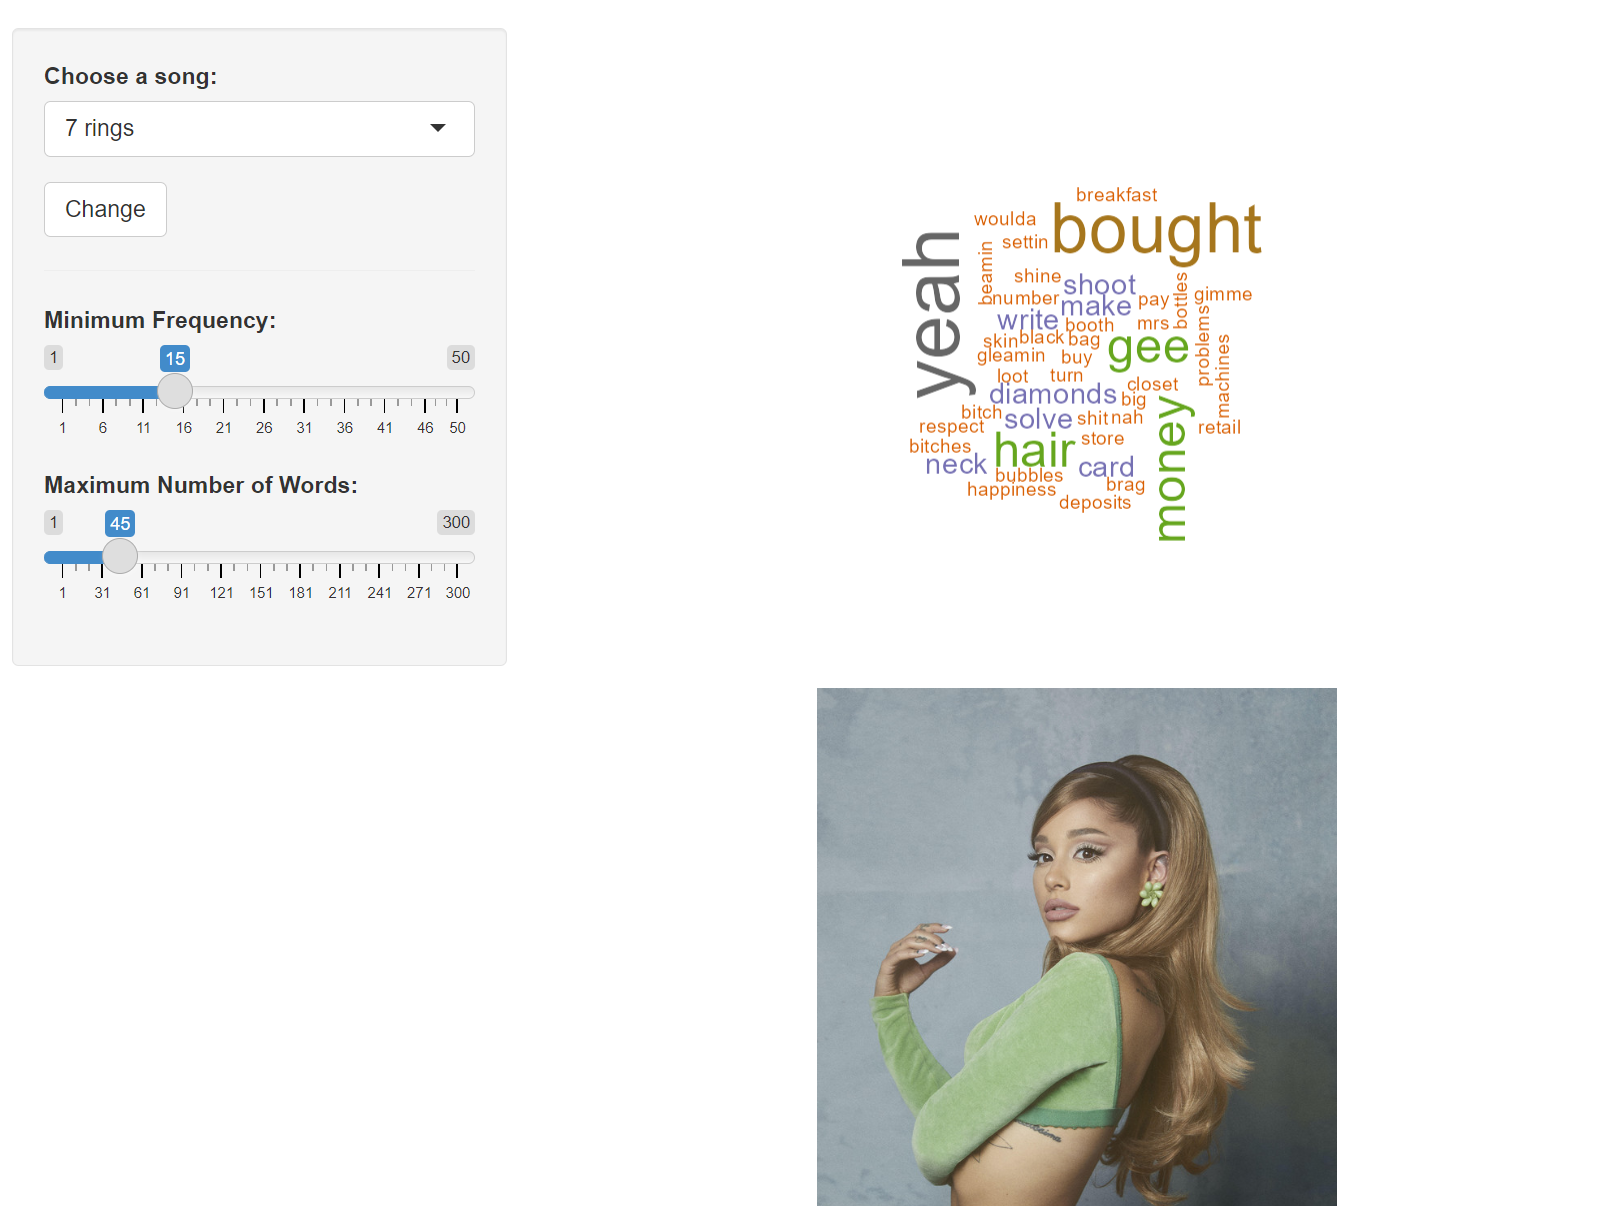
\includegraphics[width=0.75\linewidth]{Images//9_GUI/gui_wordcloud.png}
    \caption{Exemple del que es veu a l'apartat de \textit{wordcloud}}
    \label{fig:gui_wordcloud}
\end{figure}

Un altre apartat és l'encarregat de generar les playlists. Com s'ha comentat anteriorment, amb l'LSA hem sigut capaços de crear aquesta eina, i la aplicació permet que sigui molt fàcil executar-la: simplement emplenes els camps que vols i ho fa. A més, pots visualitzar la playlist de sortida d'una manera més còmode: enlloc de simplement tenir un print dels noms, veus la imatge i l'artista corresponent.

\begin{figure}
    \centering
    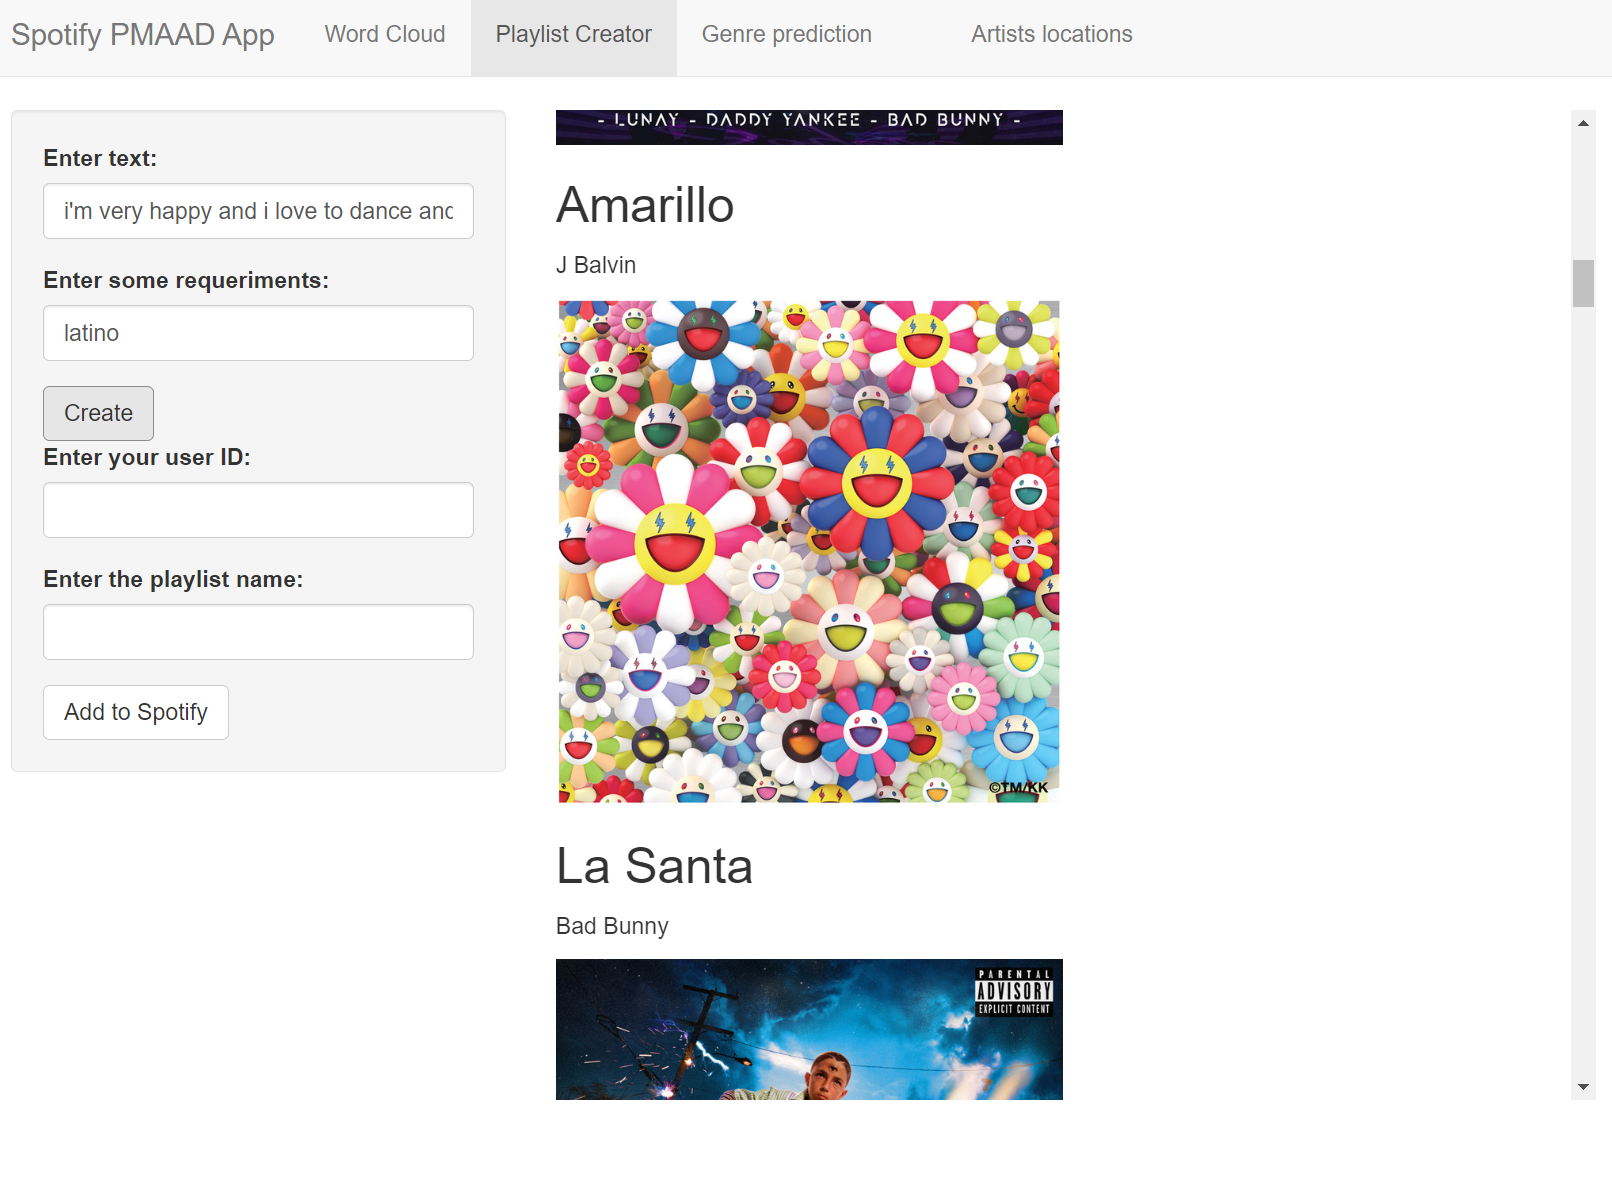
\includegraphics[width=0.75\linewidth]{Images//9_GUI/gui_playlist.png}
    \caption{Exemple de l'apartat de generació de playlists}
    \label{fig:gui_playlist}
\end{figure}

Un altre fet interessant d'aquest apartat és que, si ho desitjes, pots guardar la playlist al teu compte de Spotify. Per fer-ho, necessitaràs haver configurat abans el fitxer api\_configuration.R, amb dos \texttt{Sys.setenv}: un per SPOTIFY CLIENT SECRET i un altre per SPOTIFY CLIENT ID, les dues claus de la API. A la GUI, simplement et demana el teu UserID (que pots obtenir fàcilment quan vas al teu perfil de Spotify i copies part de l'enllaç; o bé des de configuració del perfil) i el nom de la llista de reproducció.

Hi ha un altre apartat pel predictor de gènere en funció dels lyrics, que és simplement un text box amb la sortida.

Pel que fa a geoespacials, hi ha una pestanya on pots observar un mapa del món, amb les imatges dels artistes presents al dataset i la seva ciutat de naixement. A més, et dona la opció de filtrar per gènere, per tal que puguis buscar només artistes del teu gènere preferit.

\begin{figure}
    \centering
    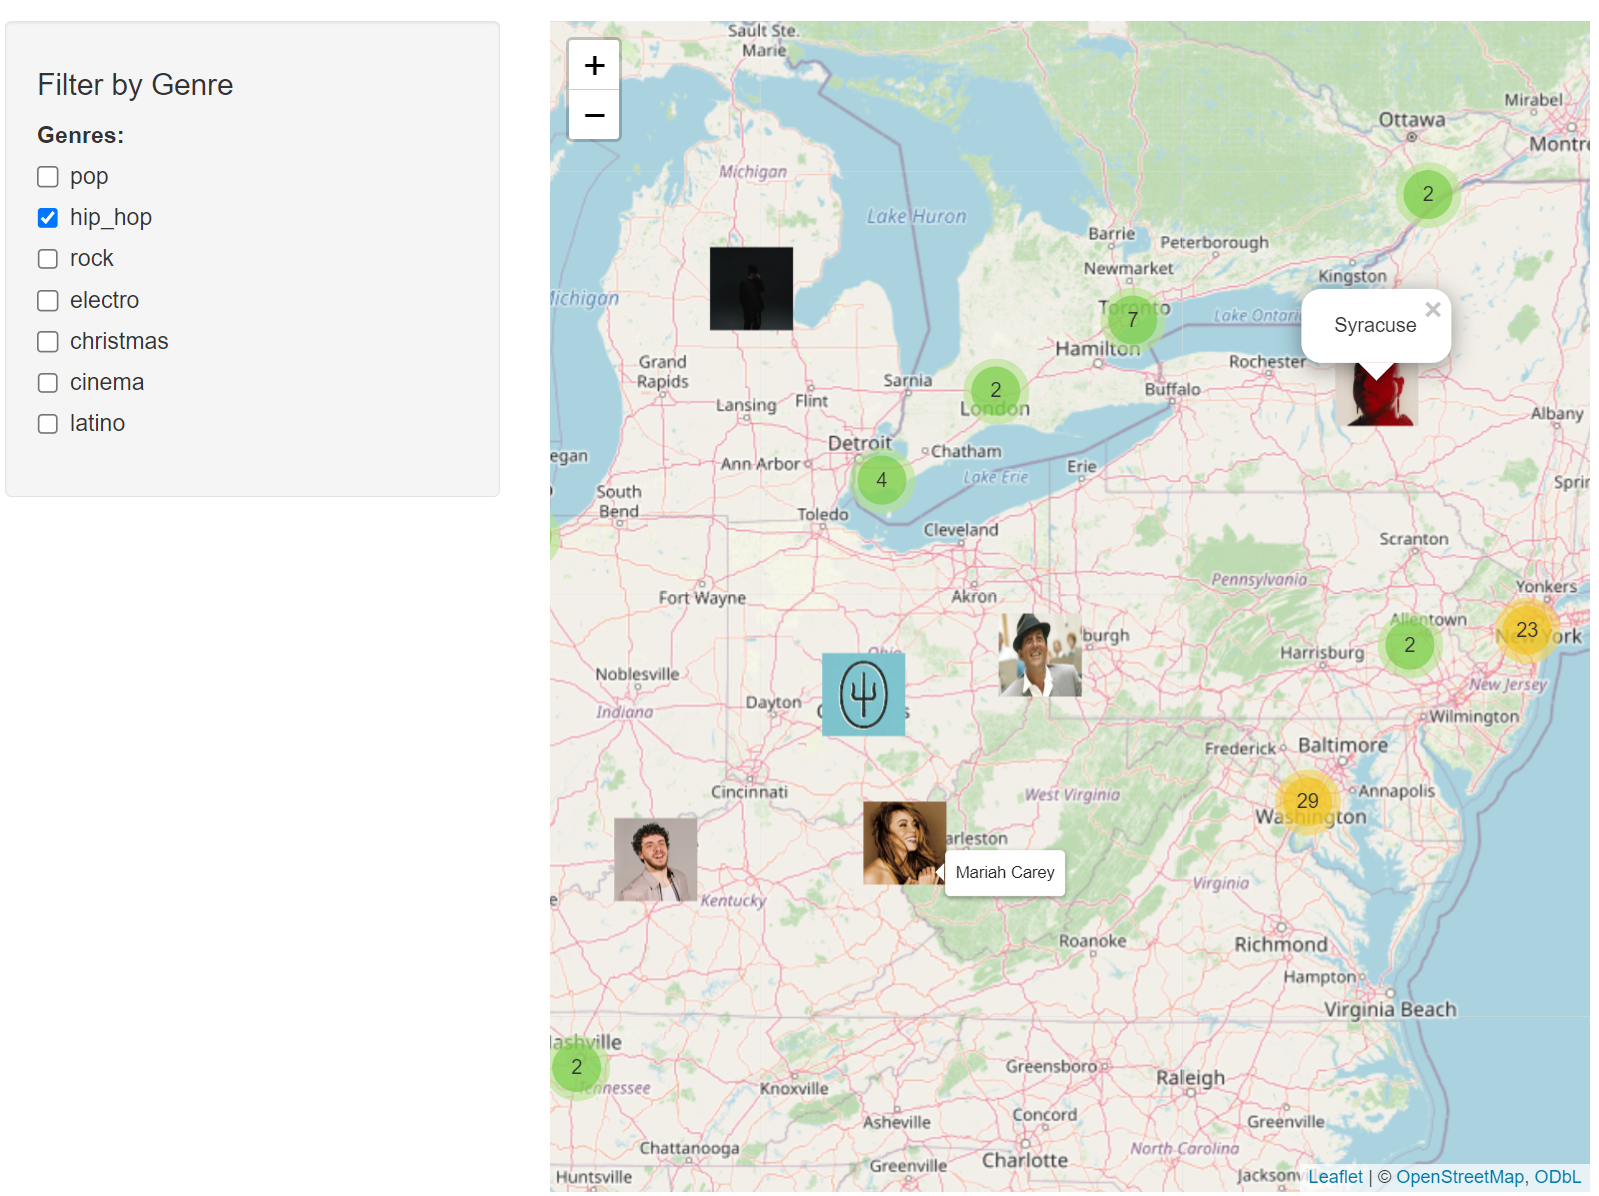
\includegraphics[width=0.5\linewidth]{Images//9_GUI/gui_map_artists.png}
    \caption{Exemple del mapa d'artistes}
    \label{fig:gui_artist_map}
\end{figure}

Addicionalment, també es va incorporar a aquesta interfície els resultats de les múltiples interpolacions amb kriging, per tal de poder clicar a qualsevol punt del món i rebre una predicció d'una cançó. Destaquem, per exemple, que si el punt clicat és de llatinoamèrica o d'Espanya, les cançons són en castellà \ref{fig:gui_geotextual}, mentre que a la resta del món són en anglès. També, per exemple, a Islàndia estan relacionades amb el Nadal; al nord del Regne Unit són de pop trist, mentre que a Londres és una de hip hop.

\begin{figure}
    \centering
    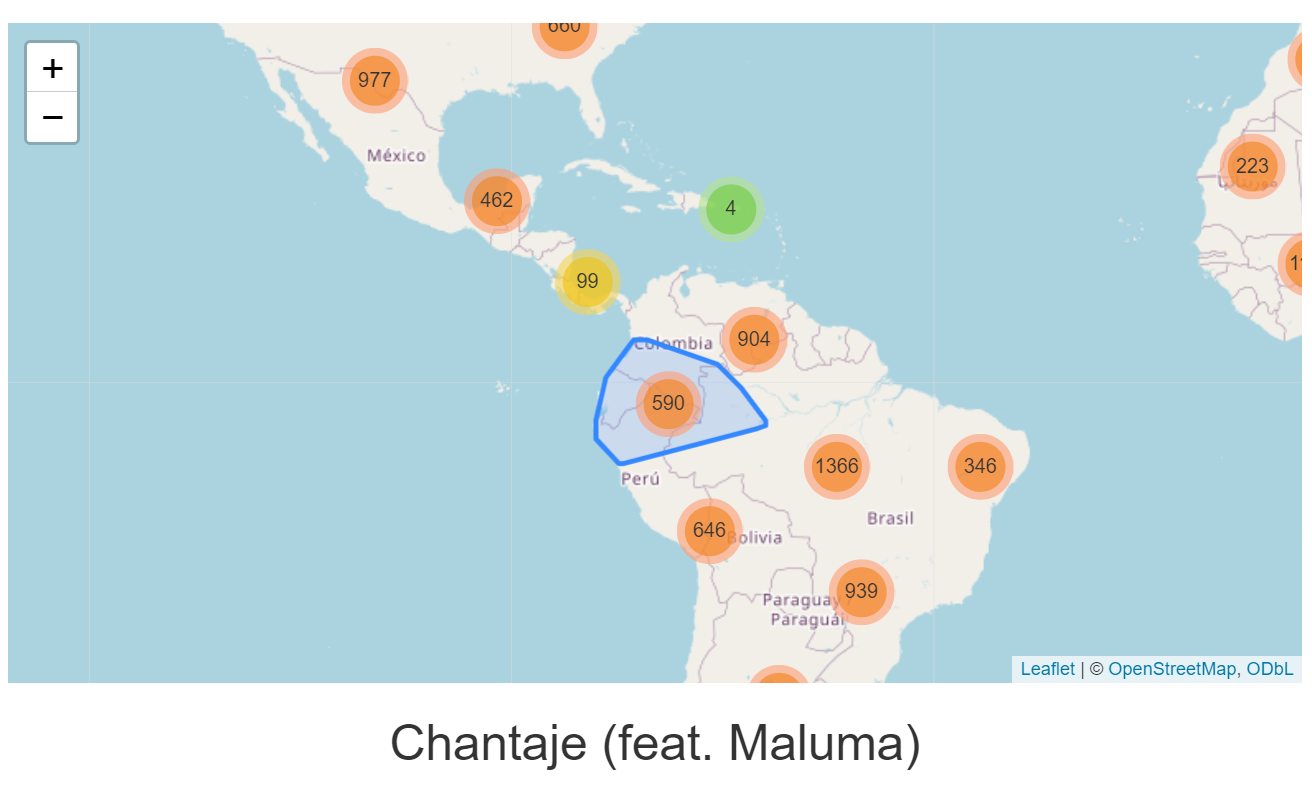
\includegraphics[width=0.75\linewidth]{Images//8_Textual//Geotextual/GUI_geotextual.png}
    \caption{Exemple de predicció en funció d'un punt}
    \label{fig:gui_geotextual}
\end{figure}

En definitiva, tot i que no era un dels objectius del treball, la interfície gràfica permet tenir un entorn on qualsevol usuari, encara que no estigui familiaritzat amb la estadística o la programació, pot interactuar amb els diferents models i visualitzacions que hem creat. Creiem que és una eina que aporta valor, i que fa més amena la interacció amb la base de dades. Al cap i a la fi, crear la interfície és un dels passos que separen un programa d'un producte que es pugui utilitzar.
